\subsubsection{Hair removal}\label{chp3-subsubsecHair}
The state of the art methods for hair detection in dermoscopy images were mentioned in Sect.~\ref{sec:chp2-sec2}.
The previously mentioned methods~\cite{Lee1997, Kiani2011,Abbas2011a,Abbas2012b,Fleming1998,Schmid-Saugeon2003,Nguyen2010,Debeir1999,Wighton2011,Chung2000,Barcelos2009,Xie2009}, were all originally proposed for hair detection and removal.
In this research, considering the similarities between hair detection and vessel segmentation in fundus images, a fast, efficient and less parametric hair detection algorithm is proposed inspired by filters proposed for vessel segmentation.
%We considered that the problem of hair detection is very similar to vessel segmentation in fundus retina images.
%Thus we considered to apply some filters and methods applied to vessel segmentation to hair detection in dermoscopy images.
From different approaches and filters, the mathematical morphological method proposed by Zana~et al.\,\cite{zana2001segmentation, giancardo2011automated} was chosen.
This algorithm is based on morphological operations, such as:
\begin{itemize}
\item[]Erosion: $\epsilon_{B}(I)$;
\item[]Dilation: $\delta_{B}(I)$;
\item[]Opening: $\gamma_{B}(I) = \delta_{B}(\epsilon_{B}(I))$;
\item[]Closing: $\phi_{B}(I) = \epsilon_{B}(\delta_{B}(I))$;
\item[]Geodesic opening (reconstruction): $\gamma_{I_{marker}}^{rec}(I_{mask})$;
\item[]Geodesic closing: $\phi_{I_{marker}}^{rec}(I_{mask}) = N_{max} - \gamma_{N_{max}-I_{marker}}^{rec}(N_{max} - I_{mask})$.
\end{itemize}
\noindent In these equations, $B$ is the structuring element, $I$ is the image, $I_{marker}$ and $I_{mask}$ are the marker and mask images respectively and $N_{max}$ is the max image where each pixel is represented by its maximum value~\cite{vincent1993morphological}.
The initial stage of this algorithm removes noise while preserving the main structure of the image.
As the algorithm intends to find bright linear structures in the image, inverted grayscale images are used as the input:
\begin{equation}
I_{op} = \gamma_{I_{0}}^{rec}(\max\limits_{i=1,2,...,n_{a}}\{\gamma_{L_{i}}(I_{0})\}),
\end{equation}
\noindent where $L_{i}$ is a linear structuring element with a constant pixel length ($p_{l}$) and different orientations defined by $i \times a_{0}$, and $a_{0}$ is the angle step ($n_{a} = \ang{360}/a_{0}$).
In this research, we set the default values: $p_{l} = 5$ and $a_{0} = \ang{10}$.
However, they can be adjusted depending on the hair density in each image.

In the next step, all the linear bright shapes in the $I_{op}$ image are obtained using: 
\begin{equation}
I_{sum} = \sum\limits_{i}^{n_{a}}(I_{op} - \gamma_{L_{i}}(I_{0})).
\end{equation}
In $I_{sum}$, the contrast of the hairs and background as well as some unwanted structures are improved.
Therefore, the author proposed filtering the image first using a Gaussian filter ($N(\mu,\sigma)$ = $N(5,1.25)$), $I_{G}$, and then applying the Laplacian operator ($W = 3 \times 3$), $I_{lap}$.
The default values can be adapted based on trial and error to suit different datasets.


Next, in the image obtained, $I_{lap}$, we remove the noise again by using geodesic opening and closing:
\begin{subequations}
\begin{align}
I_{1} & = \gamma_{I_{lap}}^{rec} (\max\limits_{i = 1:n_{a}}\{\gamma_{L_{i}}(I_{lap})\})~,\\
I_{2} & = \phi_{I_{1}}^{rec}(\min\limits_{i = 1:n_{a}}\{\phi_{L_{i}}(I_{1})\})~, \\
I_{res} & = (\max\limits_{i =1 : n_{a}}\{\gamma_{L_{i}}^{2}(I_{2})\})~.
\end{align}
\end{subequations}
The final result is achieved by thresholding the last stage $I_{res} \geq 1$.
For our purposes in the default algorithm only, the connected components with eccentricity higher than 0.87 are considered.
This value is selected since hairs are normally represented by connected lines than circles.
The components selected are dilated with a disk structure of size 3~\si{px} to create our final hair mask.
The final step is optional and can be eliminated in some cases.
%Once again, it is better to add or remove the latter morphological operations and adjust the default values according to characteristics of each image.

In order to restore the original images without hairs, we use the previously created mask and the exemplar-based inpainting method by Criminisi~et al.\,\cite{criminisi2003object}.
The exemplar-based method combines the advantage of the ``texture synthesis'' and ``inpainting'' methods.
Similar to inpainting, it pays special attention to linear structures that influence the fill order for an exemplar-based texture synthesis algorithm~\cite{criminisi2003object}.
Fig.~\ref{fig:exemplar-based} from the original paper demonstrates the main idea of this algorithm.
\begin{figure}[t]
\centering
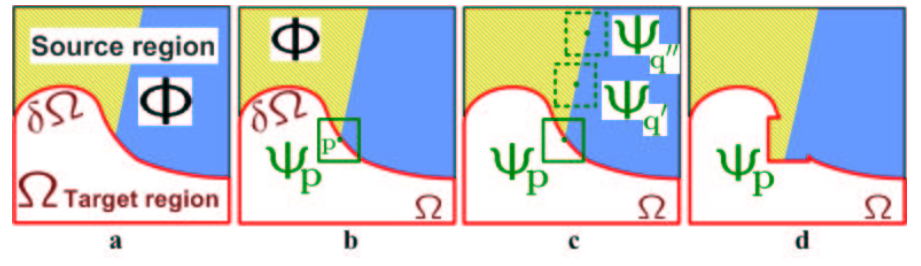
\includegraphics[scale=0.4]{Chapter3/Figures/Exemplar-based-criminisi.png}
\caption[Exemplar inpainting]{(a) Original image with target region $\Omega$, source region $\Phi$ and the contour or ``fill front'' $\delta \Omega$. (b-c) The goal is to synthesize the patch area defined by $\Psi_{p}$, using the most likely candidate ($\Psi_{q'}, \Psi_{q''}$). (d) Filling region $\Psi_{p}$ using the best matching candidate and evolving the fill front inward. This figure was taken from Criminisi~et al.\,\cite{criminisi2003object}}
\label{fig:exemplar-based}
\end{figure}

Considering the source region as the entire image minus the target region ($\Phi = I - \Omega$) and choosing a specific size of the template, all the border points are given a priority order, so that their patch region can be filled with the most similar patch from the source region.
The priority order is based on the so-called confidence term $C(p)$ and the data term $D(p)$:
\begin{subequations}
\begin{align}
P(p) & = C(p)D(p),\\
D(p) & = \vert \nabla I_{p}^{\bot}.n_{p} \vert /\alpha,\\
C(p) & = \frac{\sum\limits_{q\in\Psi_{p} \cap \Omega }C(p)}{\vert \Psi_{p}\vert},
\end{align}
\end{subequations}
\noindent where $|\Psi_{p}|$ is the area of $\Psi_{p}$, $\alpha$ is the normalization factor, $n_{p}$ is the unit vector orthogonal to the fill front ($\delta\Omega$) at point $p$, and $\nabla I_{p}^{\bot}$ illustrates the direction and intensity at this point.
After prioritizing the pixels on the border, each patch is replaced by a patch from the source region most similar to it.
The distance between two patches is based on the sum of square differences of pixels already filled in the two patches.

Fig.~\ref{fig:HairRemoval} shows some results of applying our hair removal algorithm with the default parameters.
As shown in Fig.~\ref{fig:fc} and \ref{fig:fg}, the algorithm may not be optimal if the mask detected in the first stage is not optimal.
In such cases, the optional morphological operations at the last stage of the hair detection algorithm could be removed or the default parameters adjusted.
%Since hair detection was not in the main scope of this thesis, and due to the lack of ground truth for body hair, at this point we do not have quantitative results supporting our algorithm.

\begin{figure}
\begin{center}
\subfloat[Original ]{\label{fig:fa}
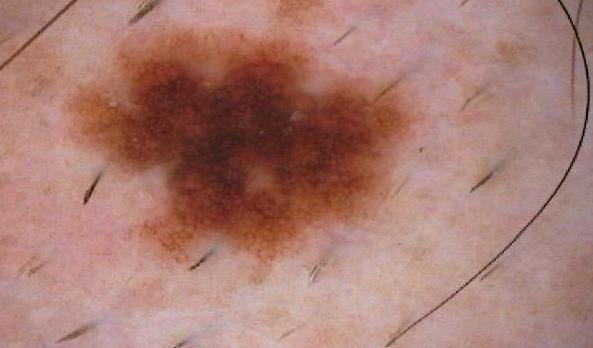
\includegraphics[width = 0.45\textwidth]{Chapter3/Figures/E1_WH_Vienna.jpg}}\
\subfloat[Restored ]{\label{fig:fb}
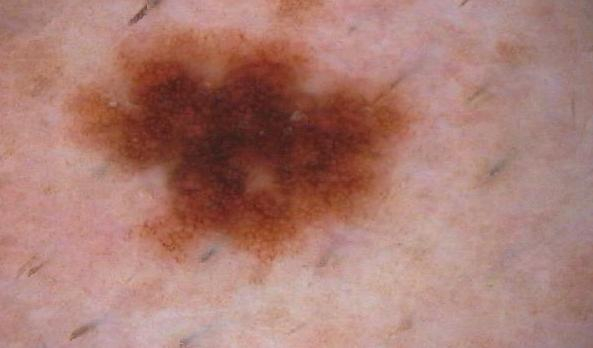
\includegraphics[width = 0.45\textwidth]{Chapter3/Figures/E1_NH_Vienna.jpg}}\\
\subfloat[Original ]{\label{fig:fc}
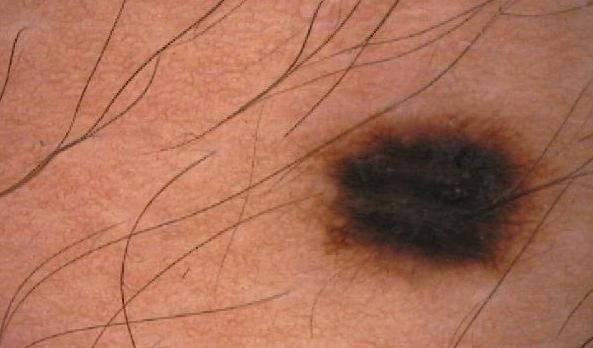
\includegraphics[width = 0.45\textwidth]{Chapter3/Figures/E4_WH_Vienna.jpg}}\
\subfloat[Restored ]{\label{fig:fd}
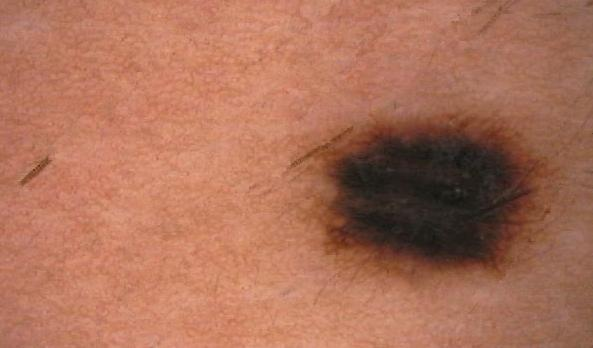
\includegraphics[width = 0.45\textwidth]{Chapter3/Figures/E4_NH_Vienna.jpg}}\\
\subfloat[Original ]{\label{fig:fe}
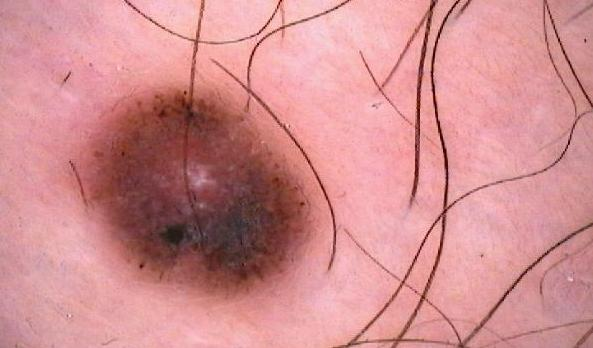
\includegraphics[width = 0.45\textwidth]{Chapter3/Figures/E5_WH_Vienna.jpg}}\
\subfloat[Restored ]{\label{fig:ff}
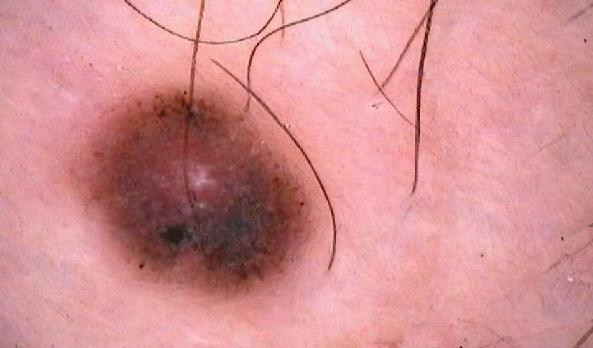
\includegraphics[width = 0.45\textwidth]{Chapter3/Figures/E5_NH_Vienna.jpg}}\\
\subfloat[Original ]{\label{fig:fg}
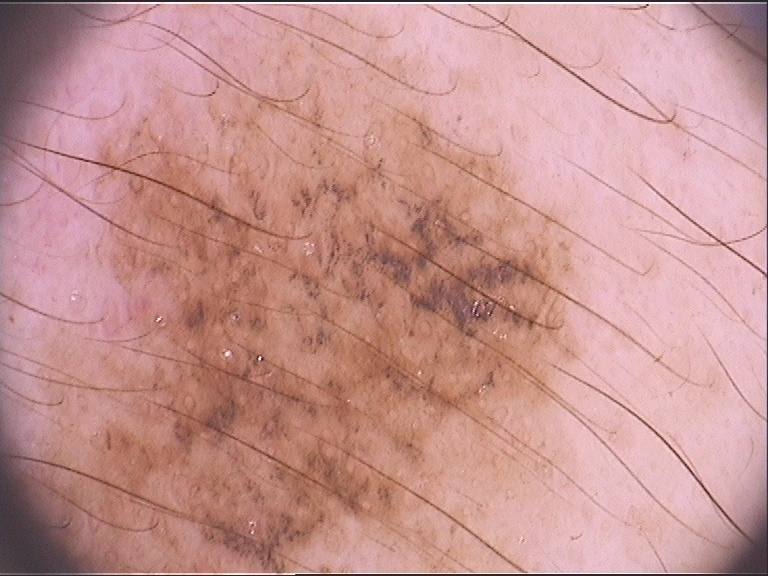
\includegraphics[width = 0.45\textwidth]{Chapter3/Figures/E1_WH_PH2.png}}\
\subfloat[Restored ]{\label{fig:fh}
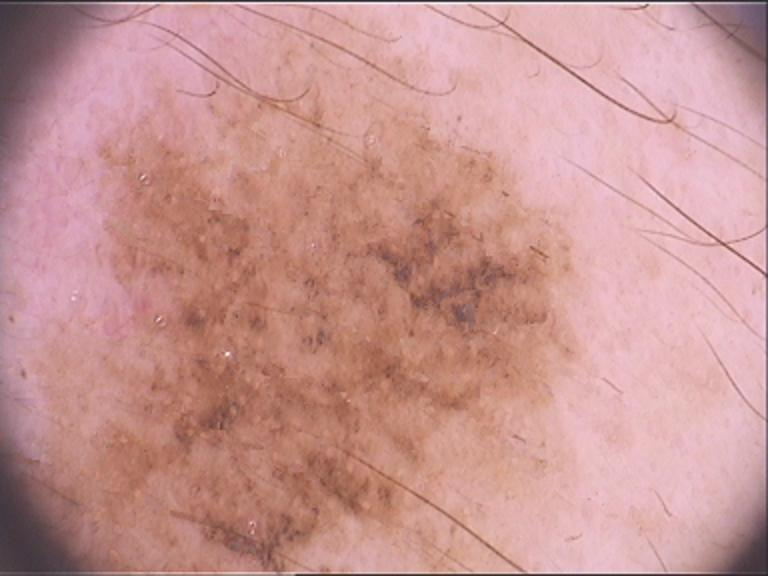
\includegraphics[width = 0.45\textwidth]{Chapter3/Figures/E1_NH_PH2.jpg}}
\end{center}
\caption[Results for the proposed hair removal algorithm]{Sample results of applying the proposed hair removal algorithm. The algorithm was used with default values for all the images. Images (a, c, e) are from the Vienna dataset and the last image (g) is from the PH$^{2}$ dataset.} %The original images are shown on the left, the images after hair removal or on the right. 

\label{fig:HairRemoval}
\end{figure}
